\documentclass[a4paper,14pt]{extarticle}
\usepackage[utf8]{inputenc}
\usepackage[russian]{babel}
\usepackage{amsmath,amsfonts,amssymb}
\usepackage{geometry}
\usepackage{graphicx}
\usepackage{url}
\usepackage[nottoc, notlof, notlot]{tocbibind}
\usepackage{listings}

\geometry{top=2cm, bottom=2cm, left=3cm, right=1.5cm}
\lstset{
    inputencoding=utf8,
    extendedchars=\true,
    literate={-}{{-}}1 {\->}{{\texttt{->}}}2 {_}{{\_}}1,
    basicstyle=\ttfamily,
    frame=single,
    captionpos=b,
}

\begin{document}

\begin{titlepage}
    \begin{center}
        Санкт-Петербургский политехнический университет Петра Великого\\
        Физико-механический институт\\[4cm]
        
        \textbf{Отчёт по лабораторной работе}\\[0.5cm]
        по дисциплине «Компьютерные сети»\\[0.5cm]
        \textbf{«Реализация протокола маршрутизации OSPF»}\\[4cm]
        
        \begin{flushleft}
            Выполнил\\
            студент гр. 5040102/30201 \hfill Завьялов И.В. \hfill \rule{3cm}{0.1pt} \\[1.5cm]
            Проверил\\
            доцент, к.ф.-м.н. \hfill \hspace{1.5cm} Баженов А.Н. \hfill \rule{3cm}{0.1pt} \\[1.5cm]
        \end{flushleft}
        
        \vfill
        Санкт-Петербург\\
        2024
    \end{center}
\end{titlepage}

\newpage

\tableofcontents

\newpage
\section{Теория}

OSPF (Open Shortest Path First) — это протокол динамической маршрутизации, основанный на технологии отслеживания состояния каналов связи (link-state). Он применяется для построения топологии сети и поиска кратчайшего маршрута между узлами с использованием алгоритма Дейкстры.

\textbf{Основные особенности протокола OSPF:}
\begin{itemize}
    \item OSPF работает с использованием метрики на основе стоимости (\textit{cost}), которая может быть основана на различных параметрах, таких как пропускная способность канала, задержка и загруженность.
    \item OSPF является внутренним протоколом маршрутизации (Interior Gateway Protocol, IGP), предназначенным для работы внутри автономной системы (AS).
    \item Протокол поддерживает иерархическую структуру сети, разделяя её на области (areas), что позволяет уменьшить размер таблиц маршрутизации и снизить нагрузку на процессор маршрутизатора.
    \item OSPF использует мультикаст-адреса (224.0.0.5 и 224.0.0.6) для передачи информации о состоянии сети между маршрутизаторами.
\end{itemize}

\textbf{Описание работы протокола OSPF:}
\begin{itemize}
    \item После включения маршрутизатора OSPF обнаруживает соседей, которые подключены непосредственно, и устанавливает с ними отношения (\textit{adjacency}). Эти отношения позволяют маршрутизаторам обмениваться информацией о сети.
    \item Каждый маршрутизатор передаёт свои данные о состоянии каналов (\textit{Link State Advertisements, LSA}) всем маршрутизаторам в той же области. Это достигается с помощью механизма \textit{flooding}.
    \item На основе полученной информации о состоянии каналов все маршрутизаторы строят одинаковую топологическую карту сети, хранящуюся в базе данных состояния канала (\textit{Link State Database, LSDB}).
    \item С использованием алгоритма Дейкстры маршрутизаторы рассчитывают кратчайший путь (\textit{Shortest Path First, SPF}) до всех других узлов сети, формируя таблицу маршрутизации.
    \item При изменении состояния сети (например, отказ или восстановление связи) маршрутизаторы обновляют свою базу данных LSDB и пересчитывают маршруты.
\end{itemize}

\textbf{Преимущества OSPF:}
\begin{itemize}
    \item Быстрая сходимость — OSPF оперативно реагирует на изменения в топологии сети.
    \item Поддержка сложных иерархических структур, что позволяет масштабировать сеть.
    \item Использование метрики, которая учитывает качество канала, позволяет выбирать оптимальные маршруты.
\end{itemize}

\textbf{Недостатки OSPF:}
\begin{itemize}
    \item Сложность конфигурации и управления в больших сетях.
    \item Значительная загрузка процессора и памяти маршрутизаторов из-за обработки LSA и расчёта маршрутов.
\end{itemize}

\section{Реализация}

\subsection{Линейная топология}
Узлы сети с линейной топологией имеют следующее расположение (рисунок 1).

\begin{figure}[htbp]
    \centering
    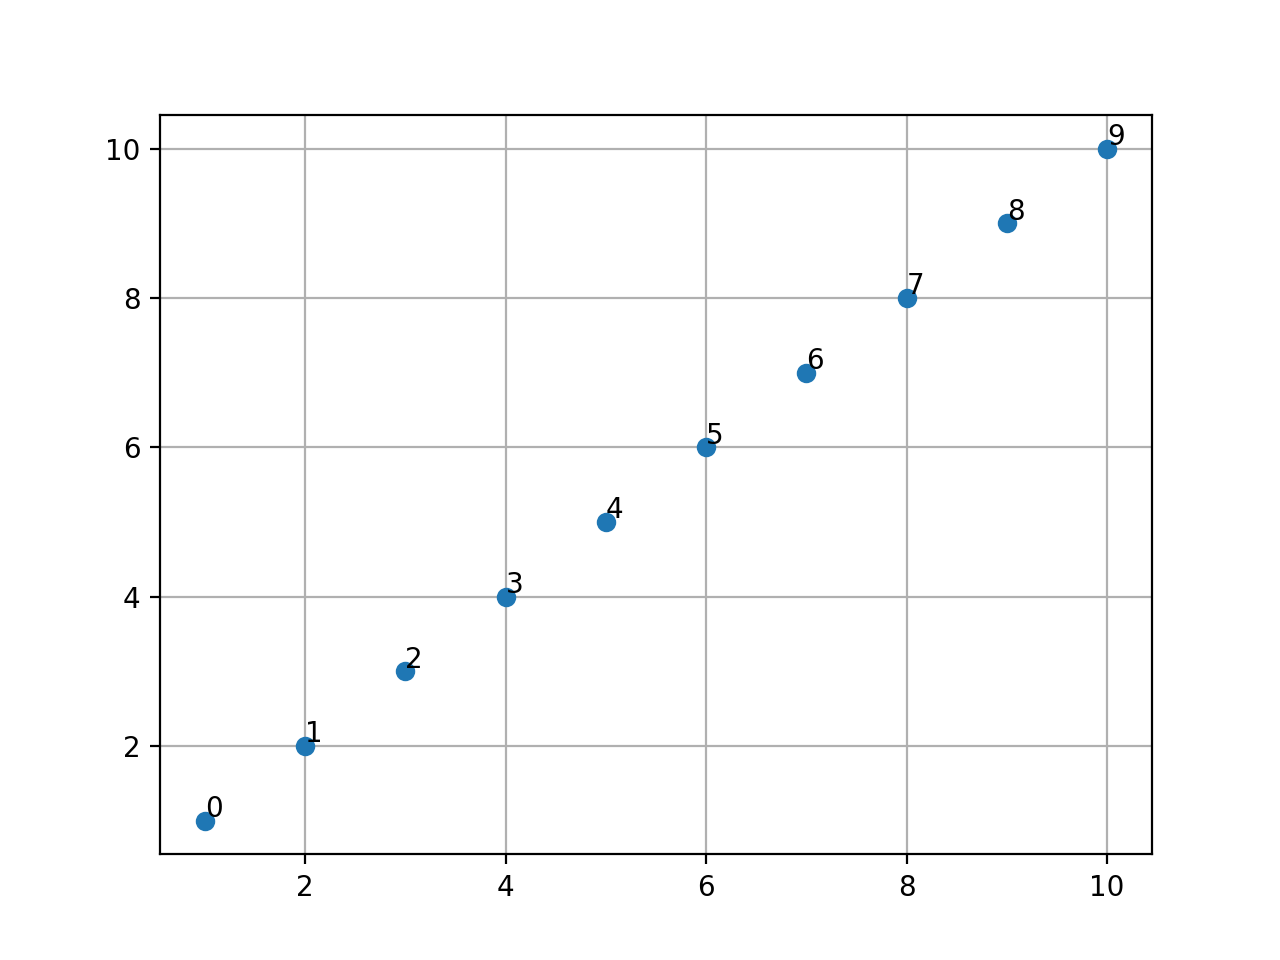
\includegraphics[width=0.8\textwidth]{img/line_points.png}
    \caption{Расположение узлов сети с линейной топологией}
    \label{fig:hamiltonianGraph}
\end{figure}

Соответствующий граф сети приведён на рисунке 2. При радиусе соединения $r=1.5$.

\begin{figure}[htbp]
    \centering
    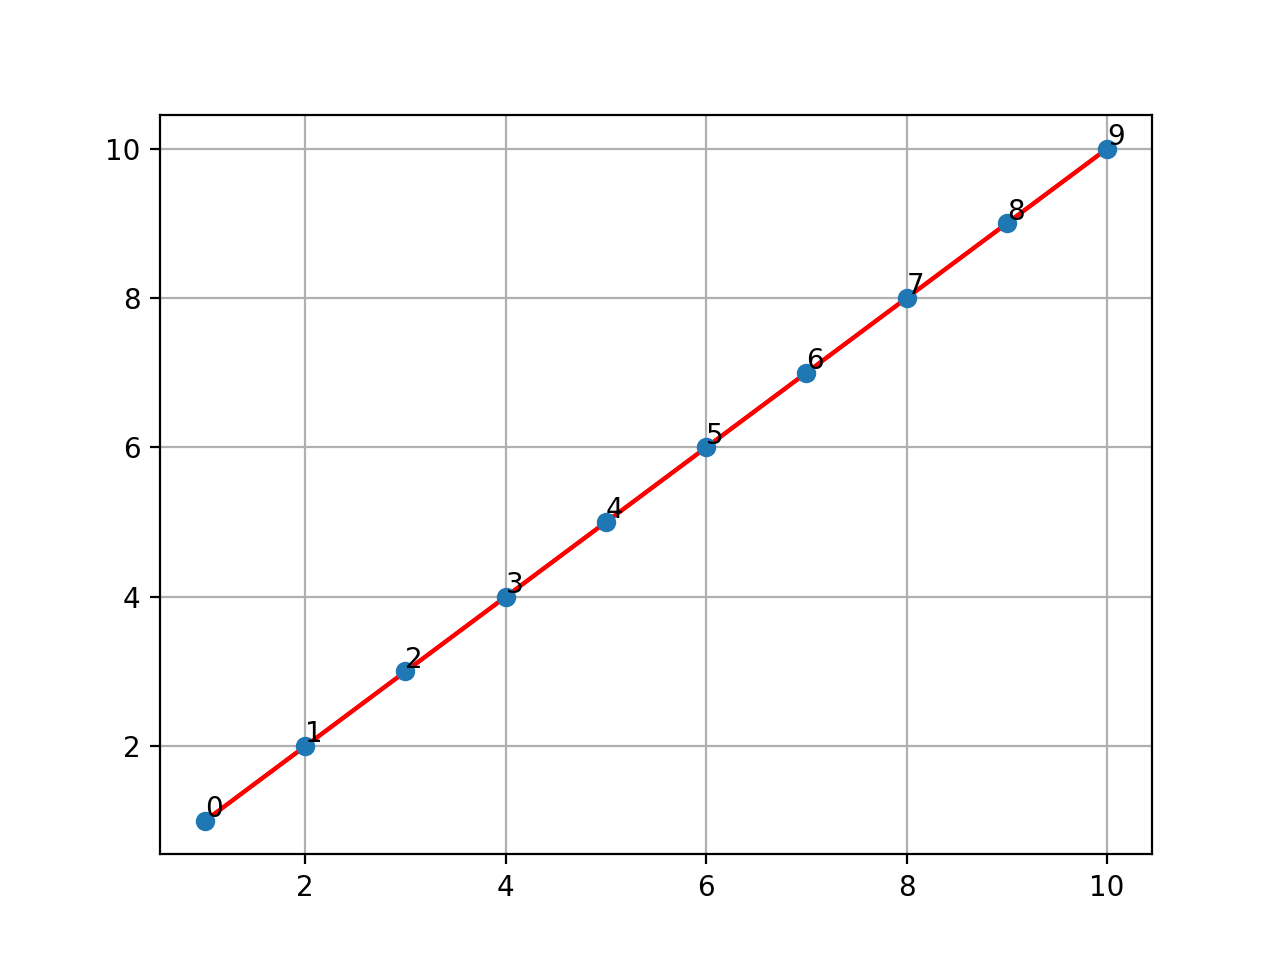
\includegraphics[width=0.8\textwidth]{img/line_graph.png}
    \caption{Граф сети с линейной топологией}
    \label{fig:hamiltonianGraph}
\end{figure}


С помощью алгоритма Дейкстры найдем кратчайшие пути от каждого узла. Результаты поиска находятся в \texttt{/path/line\_ospf.txt}.

\lstinputlisting[lastline=36, frame=single, caption=Содержимое файла line\_ospf.txt]{path/line_ospf.txt}

Пути для всех узлов приведены в файле \texttt{/path/line\_ospf.txt}.

Теперь удалим один узел из сети (например, узел 3). Тогда граф будет выглядеть следующим образом (рисунок 3).

\begin{figure}[htbp]
    \centering
    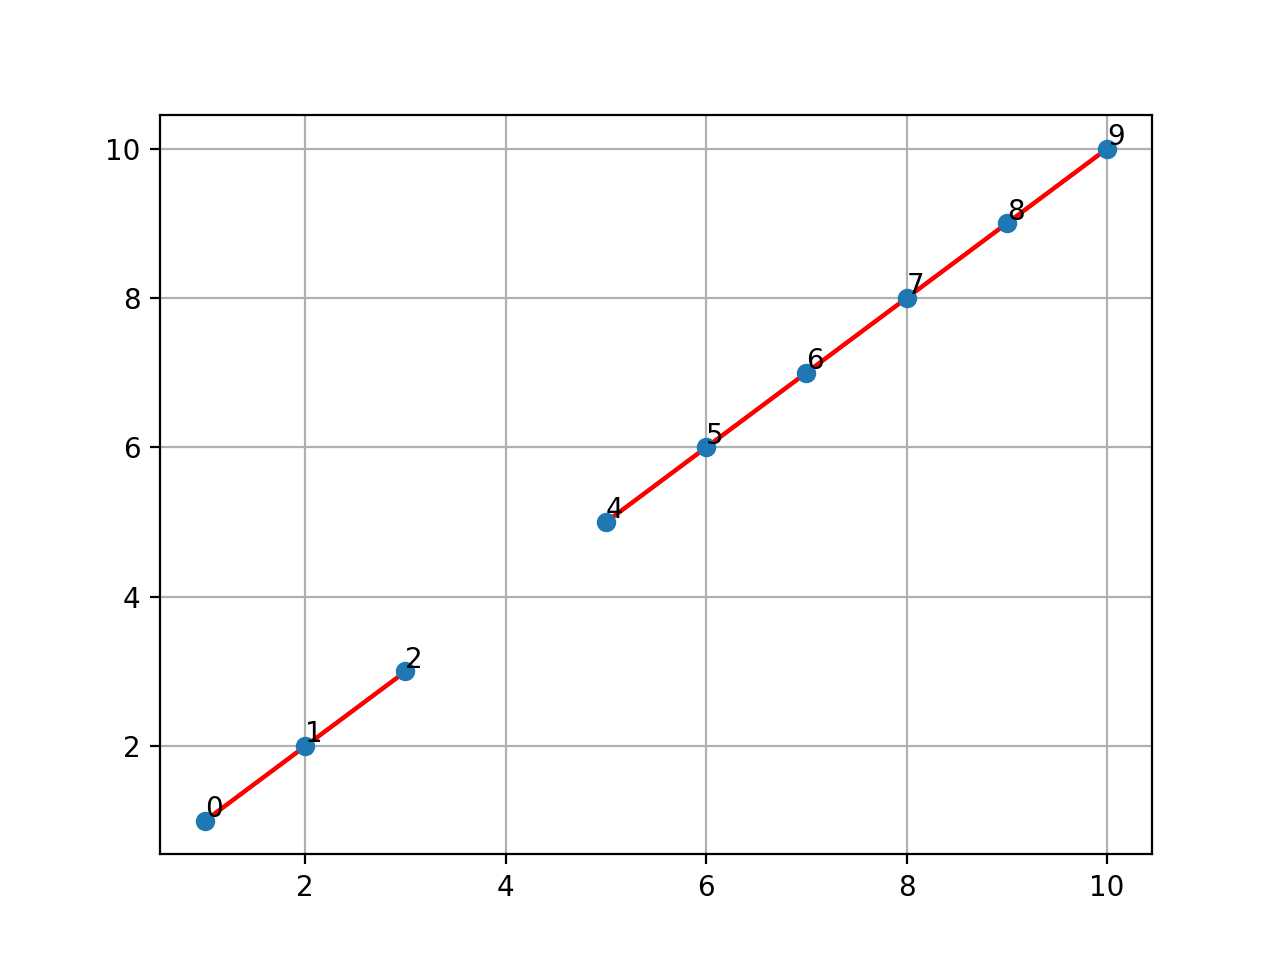
\includegraphics[width=0.8\textwidth]{img/line_modified.png}
    \caption{Граф сети с удалённым узлом}
    \label{fig:hamiltonianGraph}
\end{figure}

Найдем теперь кратчайшие пути до каждого из узлов. Результаты представлены в \texttt{/path/line\_modified\_ospf.txt}. В листинге 2 представлены пути для некоторых узлов.

\lstinputlisting[lastline=34, frame=single, caption=Содержимое файла line\_modified\_ospf.txt]{path/line_modified_ospf.txt}

\subsection{Кольцевидная топология}

Узлы сети с кольцевидной топологией имеют следующее расположение (рисунок 4).
\clearpage
\begin{figure}[htbp]
    \centering
    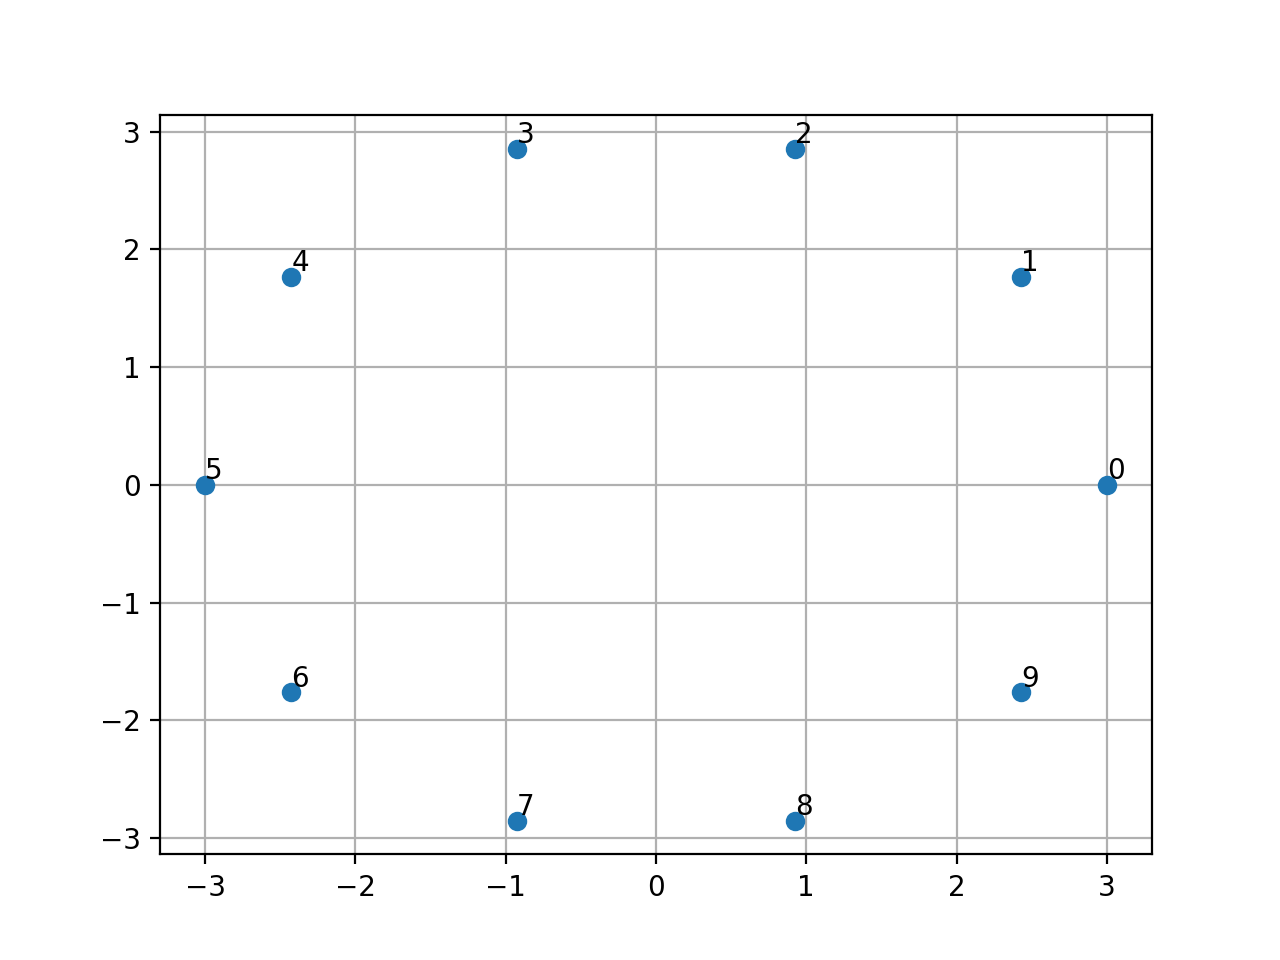
\includegraphics[width=0.6\textwidth]{img/ring_points.png}
    \caption{Расположение узлов сети с кольцевидной топологией}
    \label{fig:hamiltonianGraph}
\end{figure}


Соответствующий граф сети приведён на рисунке 5. При радиусе соединения $r=3.0$.

\begin{figure}[htbp]
    \centering
    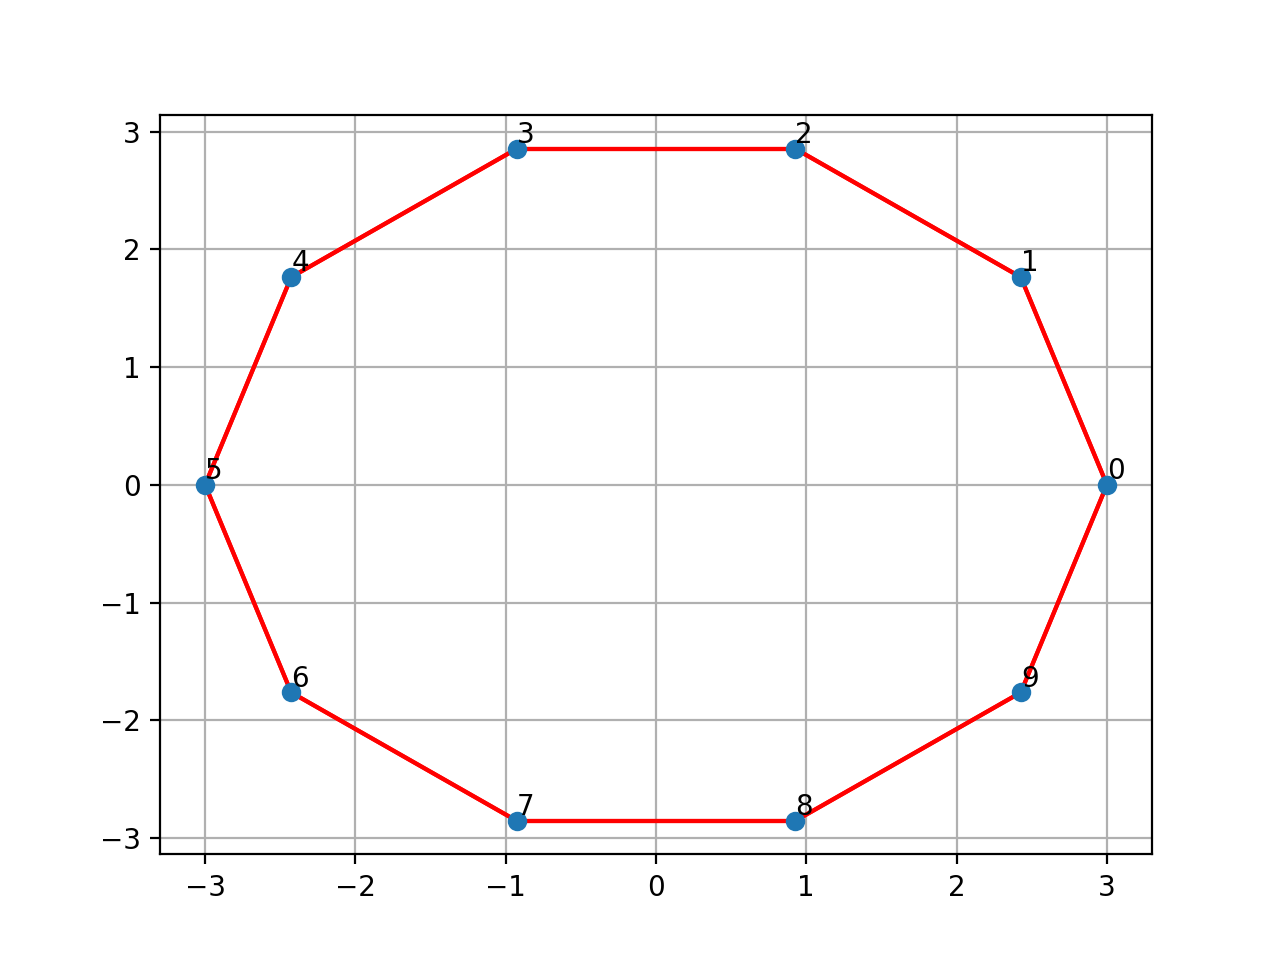
\includegraphics[width=0.6\textwidth]{img/ring_graph.png}
    \caption{Граф сети с кольцевидной топологией}
    \label{fig:hamiltonianGraph}
\end{figure}

С помощью алгоритма Дейкстры найдем кратчайшие пути от каждого узла. Результаты поиска находятся в \texttt{/path/ring\_ospf.txt}.

\lstinputlisting[lastline=36, frame=single, caption=Содержимое файла ring\_ospf.txt]{path/ring_ospf.txt}

Пути для всех узлов приведены в файле \texttt{/path/ring\_ospf.txt}.

Теперь удалим один узел из сети (например, узел 3). Тогда граф будет выглядеть следующим образом (рисунок 6).

\clearpage
\begin{figure}[htbp]
    \centering
    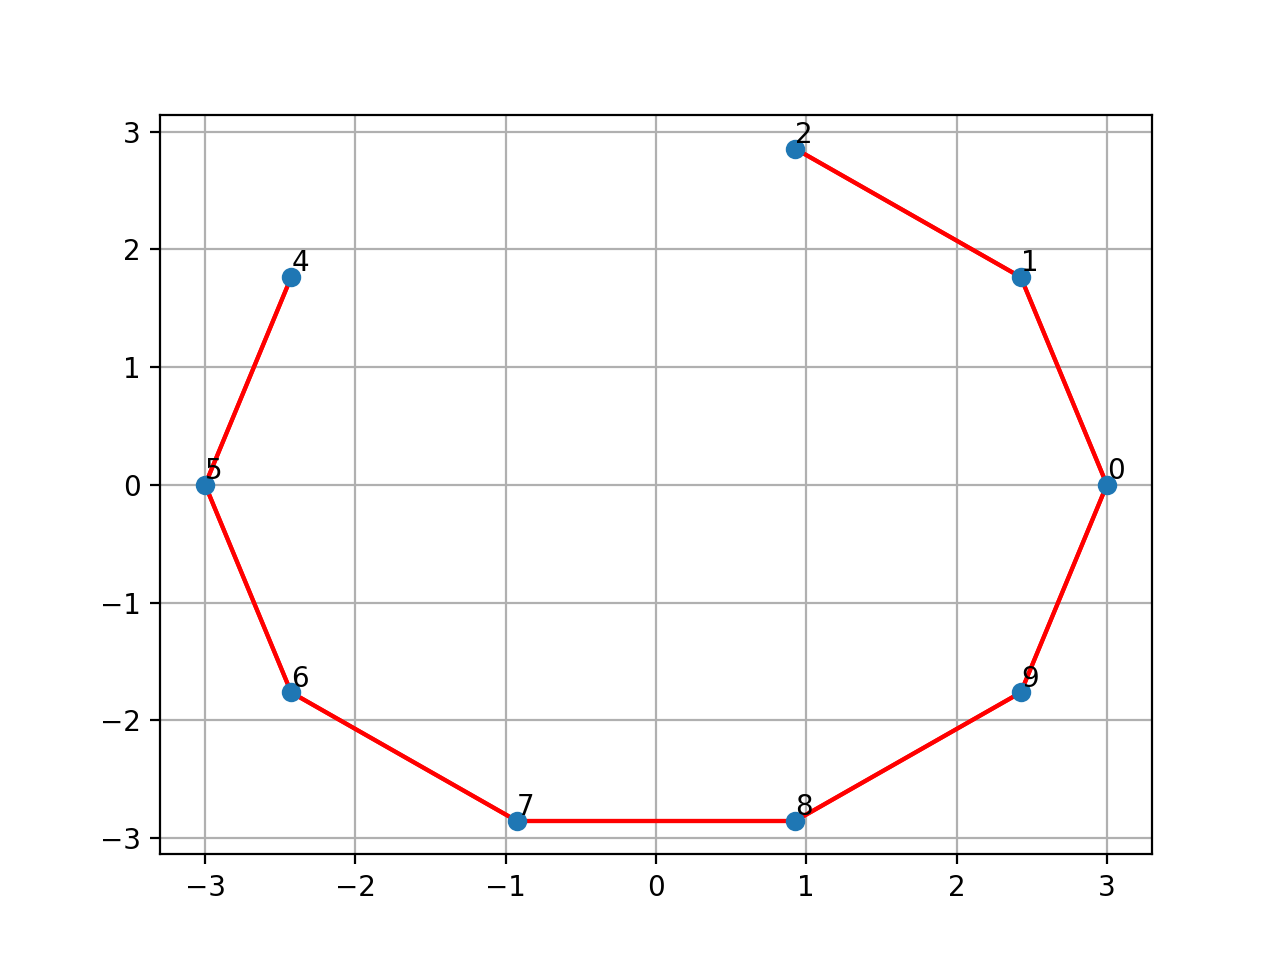
\includegraphics[width=0.8\textwidth]{img/ring_modified.png}
    \caption{Граф сети с удалённым узлом}
    \label{fig:hamiltonianGraph}
\end{figure}

Найдем теперь кратчайшие пути до каждого из узлов. Результаты представлены в \texttt{/path/ring\_modified\_ospf.txt}. В листинге 4 представлены пути для некоторых узлов.

\lstinputlisting[lastline=33, frame=single, caption=Содержимое файла ring\_modified\_ospf.txt]{path/ring_modified_ospf.txt}

\subsection{Звёздная топология}

Узлы сети с звёздной топологией имеют следующее расположение (рисунок 7).
\clearpage
\begin{figure}[htbp]
    \centering
    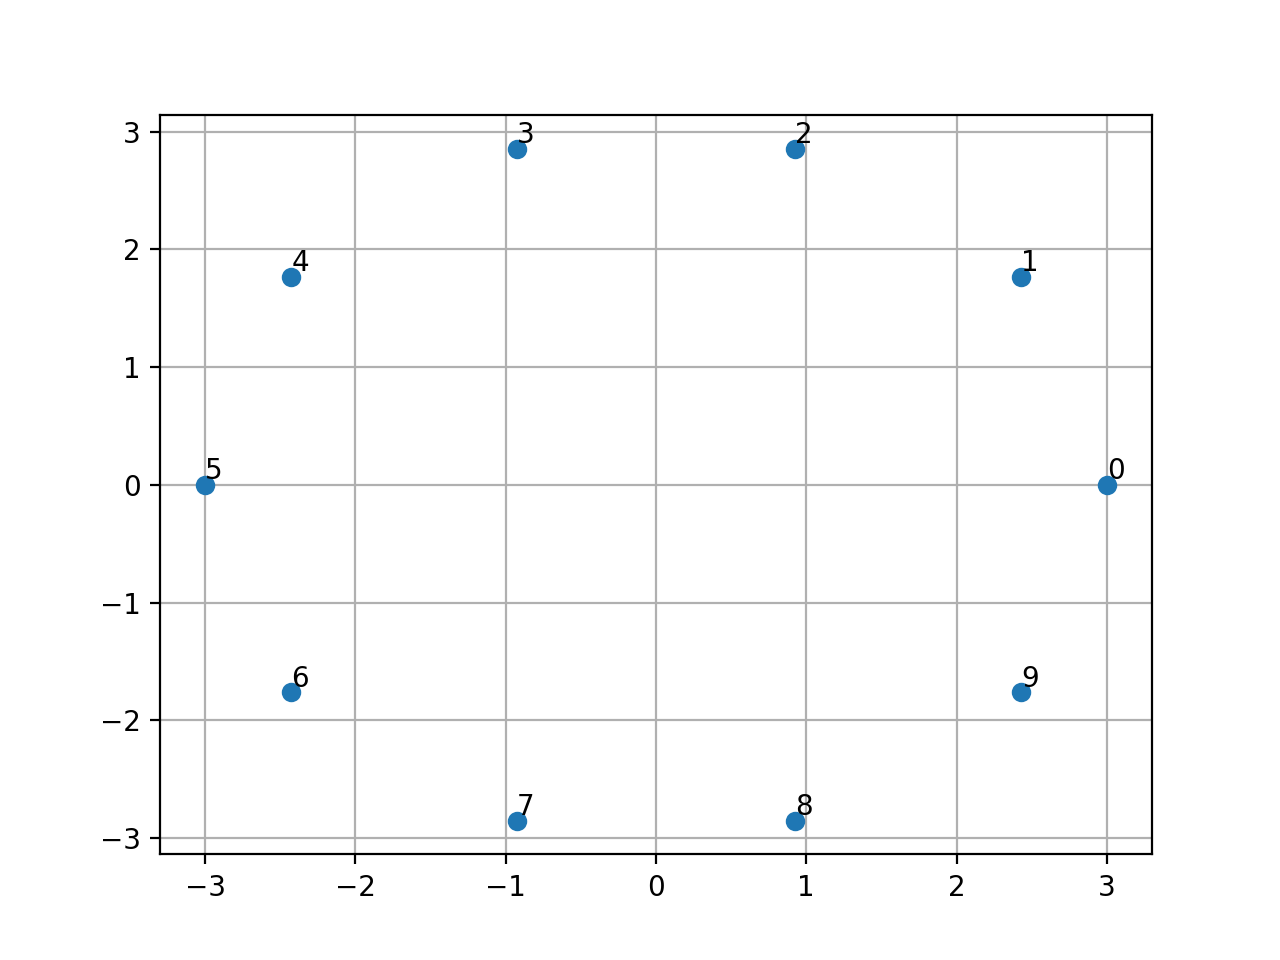
\includegraphics[width=0.6\textwidth]{img/ring_points.png}
    \caption{Расположение узлов сети с звёздной топологией}
    \label{fig:hamiltonianGraph}
\end{figure}


Соответствующий граф сети приведён на рисунке 8.

\begin{figure}[htbp]
    \centering
    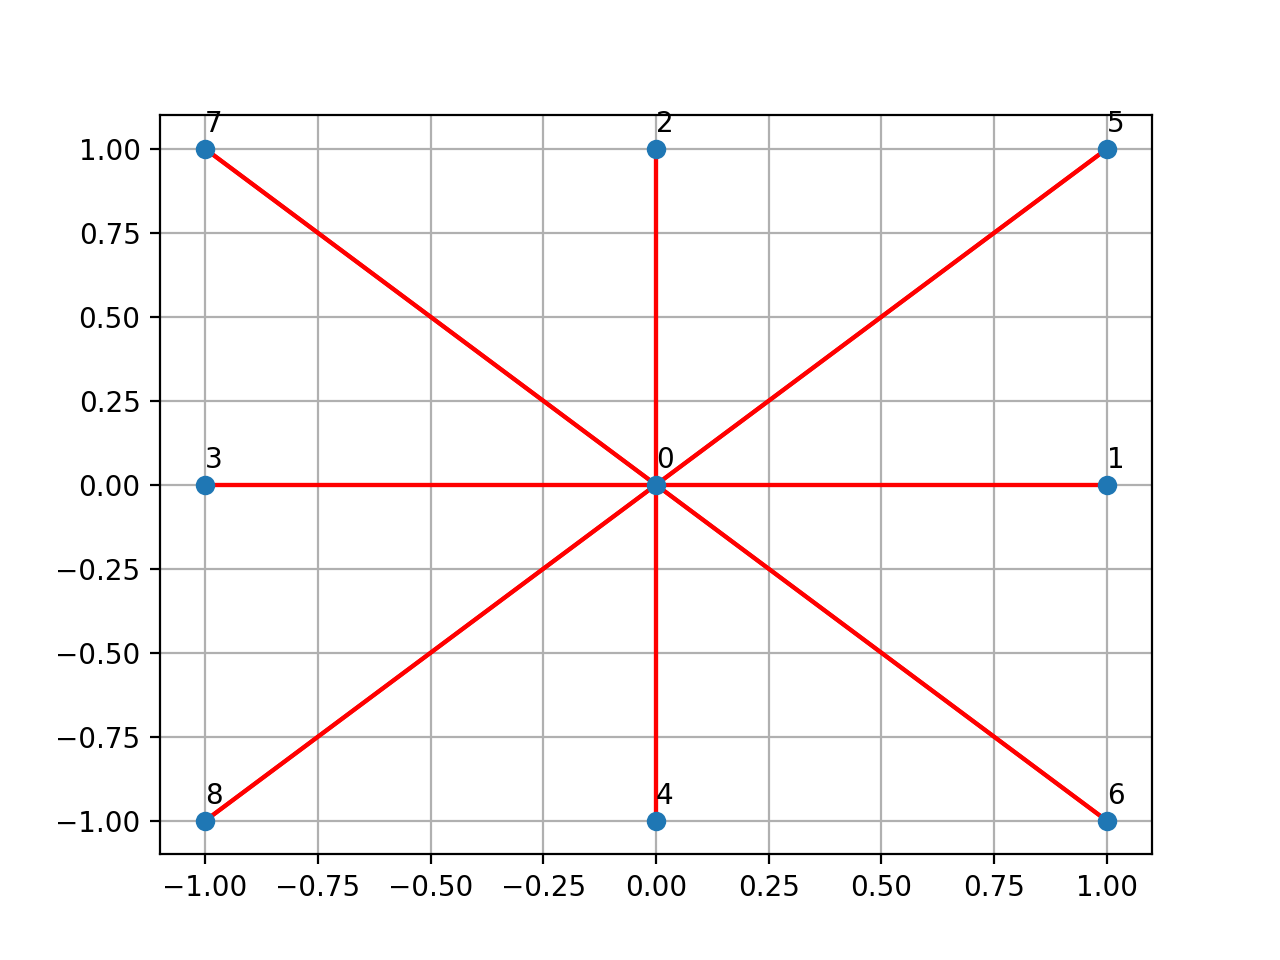
\includegraphics[width=0.6\textwidth]{img/star_graph.png}
    \caption{Граф сети с звёздной топологией}
    \label{fig:hamiltonianGraph}
\end{figure}

С помощью алгоритма Дейкстры найдем кратчайшие пути от каждого узла. Результаты поиска находятся в \texttt{/path/star\_ospf.txt}.

\lstinputlisting[lastline=36, frame=single, caption=Содержимое файла star\_ospf.txt]{path/star_ospf.txt}

Пути для всех узлов приведены в файле \texttt{/path/star\_ospf.txt}.

Теперь удалим один узел из сети (например, узел 3). Тогда граф будет выглядеть следующим образом (рисунок 9).

\clearpage
\begin{figure}[htbp]
    \centering
    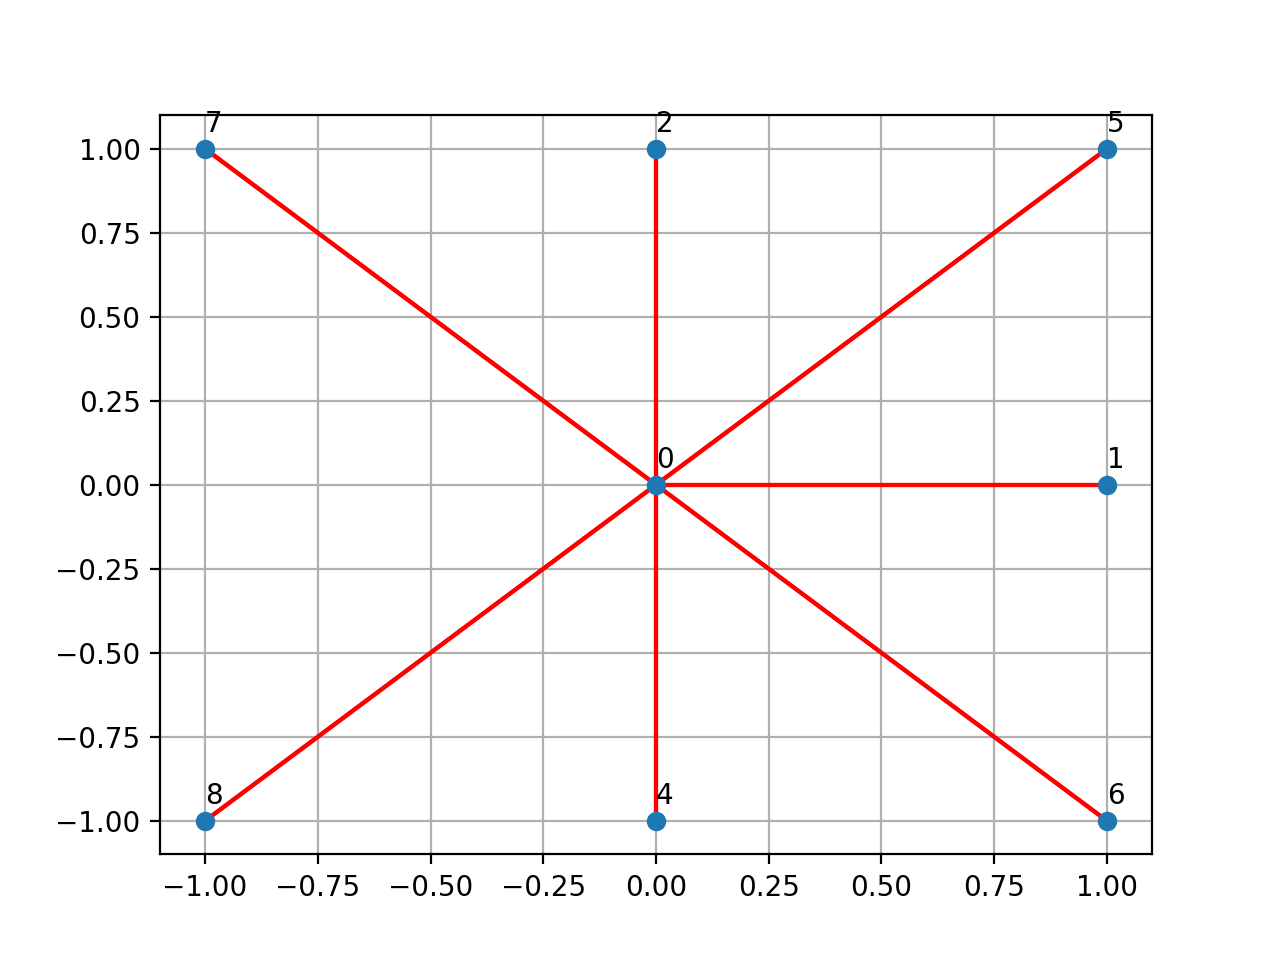
\includegraphics[width=0.8\textwidth]{img/star_modified.png}
    \caption{Граф сети с удалённым узлом}
    \label{fig:hamiltonianGraph}
\end{figure}

Найдем теперь кратчайшие пути до каждого из узлов. Результаты представлены в \texttt{/path/star\_modified\_ospf.txt}. В листинге 6 представлены пути для некоторых узлов.

\lstinputlisting[lastline=33, frame=single, caption=Содержимое файла star\_modified\_ospf.txt]{path/star_modified_ospf.txt}

\section{Выводы}

На основе проведённого анализа можно сделать следующие выводы:

\begin{itemize}
    \item Сеть с линейной топологией демонстрирует высокую уязвимость к сбоям. Потеря даже одного узла может привести к утрате связи между остальными участками сети, что значительно ухудшает её работоспособность.
    \item Кольцевая топология более устойчива к потерям узлов, так как в случае сбоя одного узла трафик может быть перенаправлен по обходному пути. Однако, если исчезает больше одного узла, кольцо разрывается, и сеть теряет свою функциональность.
    \item Сеть со звёздной топологией отличается хорошей стабильностью при отказах узлов, за исключением центрального узла. Потеря центрального узла приводит к полной потере связи между всеми остальными узлами, что делает сеть неработоспособной.
\end{itemize}
\end{document}